\documentclass[11pt,letterpaper]{article}
\usepackage[margin=1in]{geometry}
\usepackage{fontspec}
\setmainfont{TeX Gyre Pagella}
\usepackage{amsmath,amssymb}
\usepackage{unicode-math}
\setmathfont{TeX Gyre Pagella Math}
\usepackage{booktabs}
\usepackage{graphicx}
\usepackage{caption}
\captionsetup{font=small,labelfont=bf}
\usepackage{xcolor}
\definecolor{linkblue}{RGB}{0,70,180}
\usepackage[colorlinks=true,linkcolor=linkblue,citecolor=linkblue,urlcolor=linkblue]{hyperref}
\usepackage{natbib}
\setlength{\parskip}{0.35em}
\linespread{1.08}

\title{\textbf{Discrete Rules, Continuous Behavior:\\ How Judges Responded to China's 2015 Case-Registration Reform}\\[0.4em]
\large Research note --- work in progress}
\author{Zichen Fang\\ \small Peking University; visiting student, University of Chicago\\ \small \href{mailto:zcfang2025@uchicago.edu}{\texttt{zcfang2025@uchicago.edu}}}
\date{October 2026}

\begin{document}
\maketitle

\begin{abstract}
\noindent In May 2015 China replaced case \emph{screening} with case \emph{registration} in administrative litigation: courts could no longer refuse to docket suits against the government. Caseloads jumped, withdrawals fell, and procedural dismissals more than doubled. I build a dynamic model of a judge who allocates effort across mediation, adjudication, and procedural dismissal under the performance metrics Chinese courts actually use, with a backlog that links subperiods within a year and years to each other. The model is solved by nested dynamic programming and calibrated to orders of magnitude in national court statistics. In the calibrated model, the reform cuts the adjudication share of resolved cases from 66\% to 28\%, and an exact decomposition shows that the behavioral response more than offsets the mechanical effect of higher inflow on the volume of adjudicated cases. The model delivers testable predictions, including a distinctive year-end pattern, which I am now taking to case-level data built from the full archive of published Chinese court judgments.
\end{abstract}

\section{Motivation}

Before 2015, Chinese courts could informally decline to accept administrative suits, which were often politically sensitive because the defendant is a government agency. The case-registration reform, effective 1 May 2015, required courts to docket every suit that met formal requirements. Table~\ref{tab:facts} summarizes what followed, using the national tables of the \emph{China Law Yearbook}. First-instance filings rose by 59\% between 2014 and 2016 (the Supreme People's Court reports a 55.3\% increase in first-instance judgments in 2015 alone; see \citealp{ma2026}). At the same time, the share of cases closed by withdrawal fell from 30\% to 20\%, while the share closed by procedural dismissal (\emph{bohui qisu}) rose from 9\% to 22\%.

\begin{table}[h]
\centering\small
\caption{Administrative first-instance cases, national totals}\label{tab:facts}
\begin{tabular}{lrrr}
\toprule
 & 2014 & 2016 & Change \\
\midrule
Cases filed & 141,880 & 225,485 & $+59\%$ \\
Withdrawals (\% of cases closed) & 30.2 & 19.7 & $-10.5$ pp \\
Procedural dismissals (\% of cases closed) & 9.4 & 22.4 & $+13.0$ pp \\
\bottomrule
\end{tabular}
\par\smallskip\footnotesize Source: \emph{China Law Yearbook}, Table 7 (first-instance administrative cases), author's tabulation.
\end{table}

The reform removed a gate at the entrance, and the cases that came in were increasingly sent back out of the courtroom at a later stage. \citet{ma2026} document this pattern with a regression-discontinuity-in-time design on court records. This project asks \emph{why}: what in judges' incentives makes dismissal the margin of adjustment, and what does that imply for how many cases are actually adjudicated? The organizing idea is that rules change discretely while behavior adjusts continuously. A performance-evaluation system is an incomplete contract that cannot anticipate every state \citep{aghion1997}, so a reform that changes one margin (access) is absorbed through others (dismissal, mediation, effort over the year).

\section{Model}

\paragraph{Environment.} A representative judge (court) faces $N$ new cases in each of $T=4$ subperiods of a year and carries a backlog $B_\tau$. In each subperiod the judge chooses mediation effort $e_m$ and adjudication effort $e_j$, subject to the time constraint $e_m+e_j\le 1$, and a separate procedural-dismissal effort $d\in[0,1]$. A share $g(d)=1-e^{-\eta d}$ of incoming cases is dismissed; of the rest, fractions $\phi(e_m)=\phi_0 e_m^{\phi_1}$ and $\psi(e_j)=\psi_0 e_j^{\psi_1}$ are resolved by mediation and adjudication. The backlog evolves as
\begin{equation}
B_{\tau+1} = (1-\omega)B_\tau + \bigl(1-g(d_\tau)\bigr)\bigl(1-\phi(e_{m,\tau})-\psi(e_{j,\tau})\bigr)N .
\end{equation}

\paragraph{Incentives.} Courts evaluate judges on clearance and on appellate reversals, a multitask problem in the sense of \citet{hm1991}. The flow payoff is
\begin{equation}
U_\tau = w_\tau\Bigl[\bigl(\phi+\psi\bigr)\bigl(1-g(d)\bigr)N + \omega B_\tau\Bigr]
\;-\;\alpha_2\, r(e_j)\bigl(1-g(d)\bigr)\, s(e_m,e_j)
\;-\;c(e_m,e_j)\;-\;\tfrac{\delta}{2}d^2 ,
\end{equation}
where $w_\tau=\alpha_1/(TN)$ is the weight on cases closed, $r(e_j)=r_0e^{-r_1e_j}$ is the probability that an adjudicated decision is reversed (lower when more care is taken), and $c(e_m,e_j)=\tfrac{\gamma_m}{2}e_m^2+\tfrac{\gamma_j}{2}e_j^2+\gamma_{mj}e_me_j$ is a strictly convex effort cost. The key feature is the factor $s=\psi/(\phi+\psi)$, the adjudication share: reversal risk attaches \emph{only} to adjudicated cases, so mediation and dismissal are ways to escape it. This extensive margin turns out to be essential. A version without it predicts the opposite year-end pattern (Section~\ref{sec:predictions}).

\paragraph{Dynamics.} Within the year the judge solves a finite-horizon Bellman problem in $B$. At the end of the year a penalty $pB_{T+1}^2$ on the remaining backlog applies, and the backlog carries over to the next year with discount factor $\beta$:
\begin{equation}
W_\tau(B)=\max_{d}\Bigl\{-\tfrac{\delta}{2}d^2+\max_{e_m+e_j\le 1}U_\tau+\beta\,W_{\tau+1}(B')\Bigr\},\qquad
W_T(B)=\max\Bigl\{\cdots-pB'^2+\beta V(B')\Bigr\},\qquad V=W_1 .
\end{equation}
The inter-year operator satisfies Blackwell's sufficient conditions with modulus $\beta^T$, so it is a contraction with a unique fixed point $V^*$.

\paragraph{The reform.} I model registration as two changes: case inflow rises from $N=100$ to $N=150$ (the first-order effect), and procedural dismissal becomes more effective, $\eta: 5\to 8$, because courts that must docket everything shift screening to the dismissal stage (the second-order, behavioral channel). I report $N\in\{125,200\}$ as sensitivity.

\section{Solution and calibration}

The model is solved on a 51-point backlog grid and a 51-point dismissal grid. The inner effort problem is solved with an analytic Kuhn--Tucker/Newton method, cross-checked against a constrained optimizer. Inter-year value iteration converges in about 100 iterations, and the empirical contraction ratio is $0.8145=\beta^4$, matching the theoretical modulus. Before calibration I audited every analytic derivation independently: symbolic checks of first-order conditions and Hessians in SymPy, finite-difference checks of every comparative-static sign, and a clean-room re-implementation of the solver. The audit found and fixed several errors in an earlier version of the model.

Table~\ref{tab:calib} lists the calibration targets. They are orders of magnitude drawn from published court statistics rather than moments of my own data, which is the next stage of the project. Four of five targets are met. The dismissal rate is not: the model's $g(d)=0.60$ is well above the 10--25\% range. Lowering it by raising the cost of dismissal breaks the mediation share and the year-end pattern, a structural tension that I report rather than tune away. Pinning down $\eta$ and $\delta$ with case-level dismissal data is the first empirical task.

\begin{table}[h]
\centering\small
\caption{Calibration targets (pre-reform steady state)}\label{tab:calib}
\begin{tabular}{llll}
\toprule
Target & Data range & Model & \\
\midrule
Mediation share of resolved cases & 0.35--0.40 & 0.36 & \checkmark \\
Appellate reversal rate & $\approx 0.045$ & 0.040 & \checkmark \\
Year-end pattern, averaged over backlog states & --- & holds & \checkmark \\
Interior adjudication effort (no collapse) & --- & 96\% of states & \checkmark \\
Procedural dismissal rate & 0.10--0.25 & 0.60 & $\times$ \\
\bottomrule
\end{tabular}
\par\smallskip\footnotesize Calibrated parameters: $\alpha_1=0.3$, $\alpha_2=0.3$, $r_0=0.1$, $r_1=5$, $\gamma_m=0.336$, $\gamma_j=0.42$, $\gamma_{mj}=0.357$, $\phi_0=0.73$, $\psi_0=0.912$, $\phi_1=\psi_1=0.8$, $\delta=1$, $\omega=0.2$, $p=10^{-5}$, $\beta=0.95$, $\eta=5$, $N=100$.
\end{table}

\section{Results: the reform counterfactual}

\paragraph{Within the year.} Figure~\ref{fig:within} plots policies along the steady-state path. Before the reform, dismissal effort rises steadily toward year-end, while adjudication effort and the mediation share are nearly flat. After the reform, dismissal effort is higher in every subperiod and adjudication shuts down entirely in the first half of the year: every case that is not dismissed is mediated. Adjudication resumes only in the last two subperiods, when the year-end backlog penalty makes its reversal exposure worth bearing, and the mediation share falls from 1.00 to 0.41. The reform thus turns a mild within-year profile into a pronounced year-end pattern.

\begin{figure}[h]
\centering
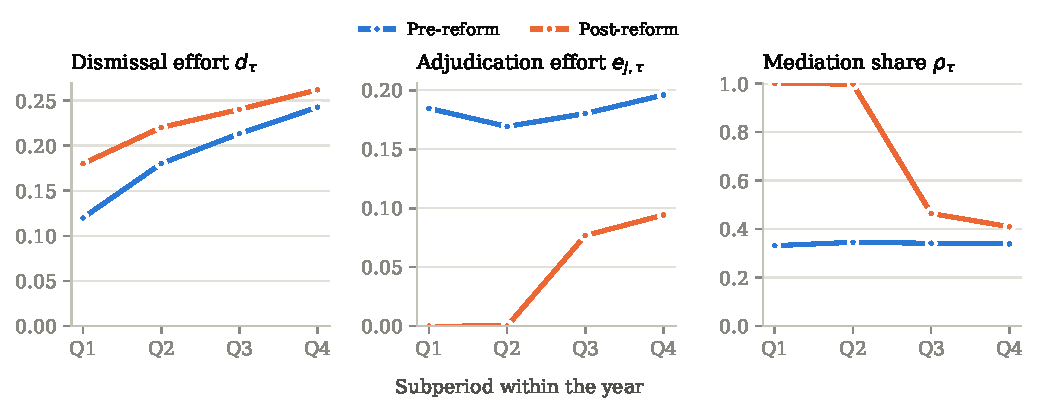
\includegraphics[width=\textwidth]{../figures/fig1_within_year.pdf}
\caption{Within-year policies along the steady state, before ($N=100,\eta=5$) and after ($N=150,\eta=8$) the reform.}\label{fig:within}
\end{figure}

\paragraph{Steady state.} Figure~\ref{fig:ss} shows the shift in how cases are resolved. The adjudication share of resolved cases falls from 0.66 to 0.28 at the central post-reform inflow, while the dismissal rate rises from 0.60 to 0.83. More inflow cushions the fall in the adjudication share but raises dismissals further: a busier court finds dismissal more worthwhile. The steady-state backlog \emph{falls} (from 122 to 98), because dismissal drains it.

\begin{figure}[h]
\centering
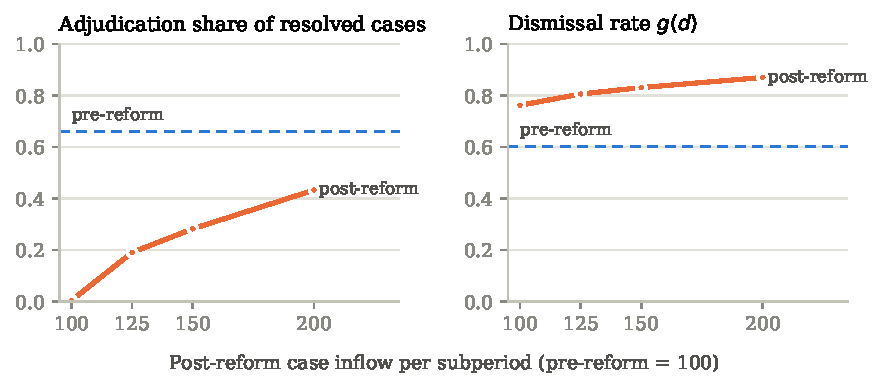
\includegraphics[width=0.86\textwidth]{../figures/fig2_steady_state.pdf}
\caption{Steady-state outcomes against post-reform case inflow ($\eta=8$). The dashed line is the pre-reform steady state.}\label{fig:ss}
\end{figure}

\paragraph{Decomposition.} Does the reform raise or lower the number of cases that actually receive a judgment? The answer is the net of a mechanical inflow effect and a behavioral displacement. Figure~\ref{fig:dec} decomposes the change in annual adjudicated volume, $\Delta V$, exactly: the components sum to the total with zero residual. The first-order inflow effect (50\% more cases at pre-reform policies) adds $+18.6$. The behavioral response subtracts more: $-15.6$ through dismissal and $-34.2$ through the collapse of adjudication effort. Additional inflow is also worth less per case once behavior has adjusted. The net effect is $\Delta V=-32.1$, so in the calibrated model displacement is 2.7 times the inflow effect. The sign is the same for $N_{\text{post}}=125$ and $200$, and the two orderings of the decomposition (behavior first or inflow first) differ only slightly. Because this prediction runs against the intuition that more access means more judgments, it is the model's sharpest point of contact with the data.

\begin{figure}[h]
\centering
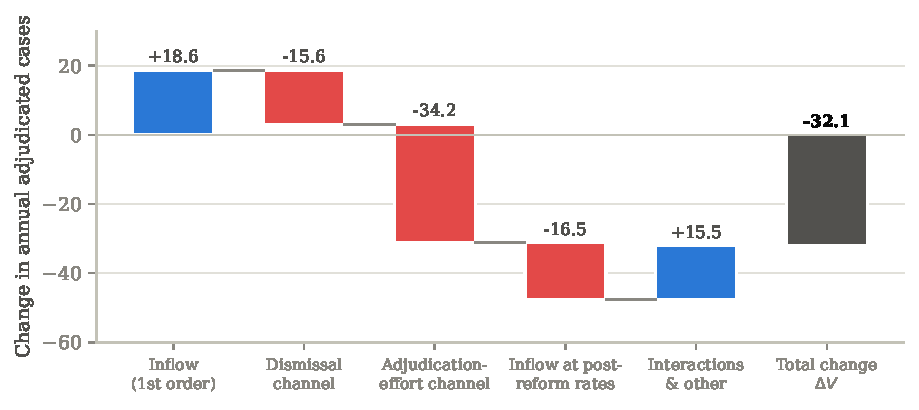
\includegraphics[width=0.8\textwidth]{../figures/fig3_decomposition.pdf}
\caption{Exact decomposition of the change in annual adjudicated volume (central case $N: 100\to150$, $\eta: 5\to8$).}\label{fig:dec}
\end{figure}

\section{Testable predictions and empirical plan}\label{sec:predictions}

The model delivers predictions that discriminate between mechanisms:
\begin{enumerate}\itemsep0.1em
\item \textbf{Exit, not entry.} After the reform, the dismissal rate rises and the adjudication share falls. The rise in dismissals is larger in higher-caseload courts.
\item \textbf{Year-end pattern.} Within a year, dismissal and adjudication effort rise toward December while the mediation share falls, and the pattern is much stronger after the reform (Figure~\ref{fig:within}). A model without the share extension predicts the opposite, a year-end surge in mediation, so monthly case outcomes separate the two.
\item \textbf{Reversal pressure pushes toward mediation.} Courts facing stronger reversal penalties shift from adjudication toward mediation, and more so when the backlog is low.
\item \textbf{Immediate response.} Dismissal behavior responds in the reform year itself rather than with a multi-year lag.
\item \textbf{Net adjudicated volume.} The decomposition in Figure~\ref{fig:dec} gives the inflow and displacement components as targets for estimation.
\end{enumerate}

\paragraph{Data.} (i) National and provincial tables from the \emph{China Law Yearbook}, 2002--2022, which I have digitized and structured. (ii) The full archive of judgments published on China Judgments Online, 1985--2021, which records case type, procedure, court, dates, cited statutes, and full text. (iii) A hand-coded set of 60 administrative cases, built at the start of the project, that serves as the seed set for classifying case outcomes and dismissal grounds from text.

\paragraph{Next steps.} (1) Build case-level outcome variables (dismissal, withdrawal or mediation, judgment, and the stated grounds) from the judgment texts, validating the classifier on the hand-coded cases. (2) Aggregate to a court-by-month panel and test predictions 1--4, using the reform date for event-study and RDiT comparisons and cross-court variation in caseload. (3) Estimate the structural parameters by simulated method of moments, with the dismissal rate as the first moment to discipline.

\paragraph{Limitations.} The model has a single representative judge and treats plaintiffs' entry as exogenous within the year. The reform is represented by two parameter changes rather than derived from a model of screening. Several calibration targets are aggregate orders of magnitude rather than moments for administrative cases specifically.

\bibliographystyle{apalike}
\begin{thebibliography}{9}
\bibitem[Aghion and Tirole(1997)]{aghion1997} Aghion, P., and J. Tirole (1997). Formal and real authority in organizations. \emph{Journal of Political Economy}, 105(1), 1--29.
\bibitem[Holmstrom and Milgrom(1991)]{hm1991} Holmstrom, B., and P. Milgrom (1991). Multitask principal--agent analyses: Incentive contracts, asset ownership, and job design. \emph{Journal of Law, Economics, \& Organization}, 7, 24--52.
\bibitem[Ma and Cheng(2026)]{ma2026} Ma, C., and C.-Y. Cheng (2026). Embedded courts under campaign-style enforcement: How top-down reforms reshape conditional justice in China. \emph{International Review of Law and Economics}, 86, 106331.
\end{thebibliography}

\end{document}
